\subsection{CMOS Device Model: Equivalent Circuit Decomposition + Dynamic Parameters}\label{subsec:cmos-model}
As mentioned earlier, any subcircuit module (e.g., CMOS) that satisfies Assumption \ref{assumption:intrinsic-params-dependencies} can be modeled as a submodel-based representation featuring "equivalent circuit decomposition + dynamic parameters". This section provides an implementation example based on a lookup table. Reimplementing BSIM model \cite{chauhan2012bsim} as a SubModel is a conventional method that offers better compatibility with the existing method, but it is not adopted in this work. The CMOS module definition consists of the following elements (details about the definition are provided in Appendix \hyperref[appendix:mos-subckt]{B} and the equivalent circuit diagram under AC analysis is given in Figure \ref{fig:mos-small-signal-model-2}):
\begin{enumerate}[partopsep=0pt,topsep=0pt,itemsep=0pt,parsep=0pt]
  \item Internal and external nodes: \textbf{nodes}=[gate,source,drain,bulk];
  \item Input parameters for the device size: \textbf{ip}=[MosL,MosW];
  \item Intrinsic parameters output by SubModel:
    \textbf{intrp}=[ID,GDS,CDD,CSS,CGG,CGS,CGD, GM,GMB], whose value is determined by the four bias voltage values (\textbf{nodes}) and device size (\textbf{ip}).
\end{enumerate}
The compiler loads external libraries and generates a function object of class "lut.MosLookup" to register it as a submodel in the subcircuit rule (Table \ref{tab:BasicCompositeSubCktRule}). Among the intrinsic parameters, ID indicates the DC current between source and drain under DC analysis, and GDS, CDD, GM, etc. are equivalent small-signal parameters under AC analysis.
\begin{figure}[htpb]
  \centering
  
\includegraphics[width=0.7\textwidth]{fig/mos-small-signal-model-2.pdf}
  \caption{CMOS equivalent small-signal model \cite[Figure 2.39]{razavi2002design}, where, Ro is a resistor with resistance $\frac{1}{\text{GDS}}$.}
  \label{fig:mos-small-signal-model-2}
\end{figure}
There are a few points to note:
\begin{enumerate}[partopsep=0pt,topsep=0pt,itemsep=0pt,parsep=0pt]
  \item The role of built-in basic elements ICS and ACVCCS (Appendix \hyperref[appendix:mos-subckt]{B}) is to ensure that ID only functions under DC analysis, while GDS, GM and GMB only function under AC analysis.
  \item The DCAC hybrid analysis or DC analysis computational graph of the equation constructor can execute this circuit module. However, the pure AC analysis computational graph cannot independently run this circuit module: In order to establish the AC analysis equations, it is necessary to first compute [GDS,GM], etc., which are determined by the DC bias voltage. This is different from directly inducing small signal linear equations through TRAN analysis equations (Appendix \hyperref[appendix:TRAN-to-AC-equation]{A}). In fact, Assumption \ref{assumption:intrinsic-params-dependencies} also stipulates that internal variables can depend on the bias voltage signal, but not on the small signals in linear analysis.
  \item The SubModel can freely call external programs, such as using three-dimensional spline interpolation, provided that it ensures compliance with the interface requirements of the corresponding automatic differentiation system.
\end{enumerate}
This submodel-based device model representation method features "equivalent circuit decomposition + dynamic parameters" and shows the following advantages:

\begin{enumerate}[partopsep=0pt,topsep=0pt,itemsep=0pt,parsep=0pt]
  \item Decoupled from circuit network analysis or simulation, the submodel is only responsible for calculating the intrinsic parameters and Jacobian matrix (Section \ref{subsec:subckt-instance-data-structure}). Circuit connectivity is not the submodel's concern.
  \item The syntax and capability boundary of a submodel in calculating intrinsic parameters depend on the compiler's processing of the "SubModel" field in the netlist. This can be implemented easily using various external programs and automatic differential tools.
\end{enumerate}

\subsection{OpAmp Device Sizing: DC Operating Points Optimization Under Different PVT Combinations}
Figure \ref{fig:manually-design} shows the device sizing process in analog circuit design. Specifically, designers connect available devices accessible to the target process into circuits, and adjust the size of each device (such as a CMOS device) based on specific methodologies and experience so that a circuit can fulfill specification requirements under a given area and power consumption constraints. In this process, repeated circuit simulation is done to quantitatively inspect the behavior and performance of a circuit without the need to manufacture the physical circuit.
\begin{figure}[htpb]
  \centering
  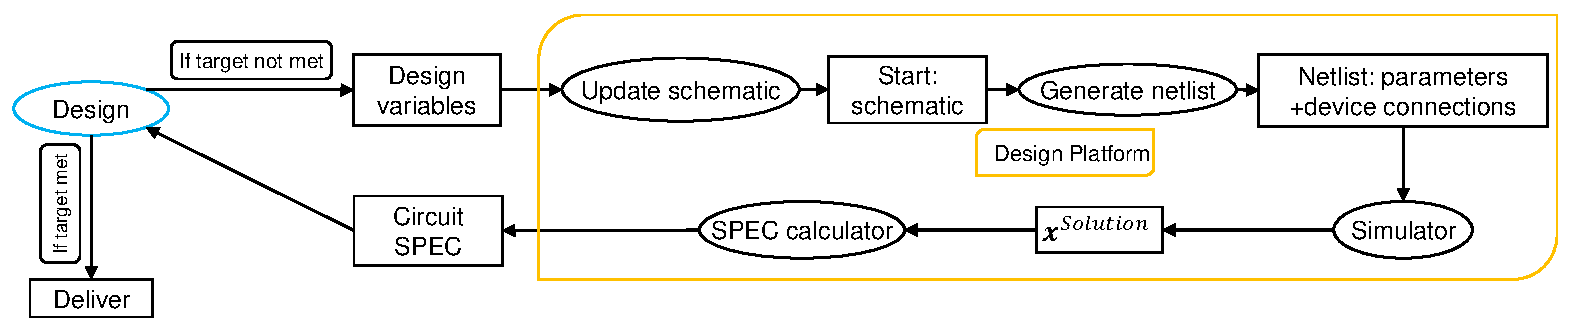
\includegraphics[width=\textwidth]{fig/manually-design.pdf}
  \caption{Manual device sizing: an iterative process}
  \label{fig:manually-design}
\end{figure}

This process can be naturally converted into an optimization problem. The optimization strategy varies depending on whether the gradient is acquirable \cite{zhan2004optimization,agrawal2006circuit,huang2013efficient,nieuwoudt2005multi,peng2016efficient,girardi2011analog,lyu2018batch,wang2014enabling,lyu2017efficient,tang2018parametric}. Take DC simulation as an example. To obtain the gradient, the DC steady-state equations $\bm{F}(\bm{x},\bm{p})=\bm{0}$ naturally provide an implicit mapping from the parameter $\bm{p}$ to the solution $\bm{x}^{solution}$ of the systems of equations, with the Jacobian matrix of this mapping being $\nabla_{\bm{p}}\bm{x}^{solution}=-\nabla_{\bm{x}}\bm{F}\backslash\nabla_{\bm{p}}\bm{F}$, where $\nabla_{\bm{x}}\bm{F},\nabla_{\bm{p}}\bm{F}$ may be directly given by the equations system construction method (computational graph \ref{fig:computational-graph}) described in Section \ref{sec:Joanna}.
With this information, the gradient optimization method (Figure \ref{fig:solve-then-optimize}) can be used.
Note that in an optimization process, the inverse of $\nabla_{\bm{x}}\bm{F}$ does not need to be completely solved.
Instead, it is sufficient to solve a set of linear equations only once during each iteration's gradient backpropagation for a given loss function or constraint function $l$:
$\nabla_{\bm{p}}l(\bm{x}^{solution})=(\nabla_{\bm{p}}\bm{x})^T\cdot\nabla_{\bm{x}}l
=-(\nabla_{\bm{p}}\bm{F})^T\cdot\big(\nabla_{\bm{x}}\bm{F}^T\backslash\nabla_{\bm{x}}l\big)$
\begin{figure}[htpb]
  \centering
    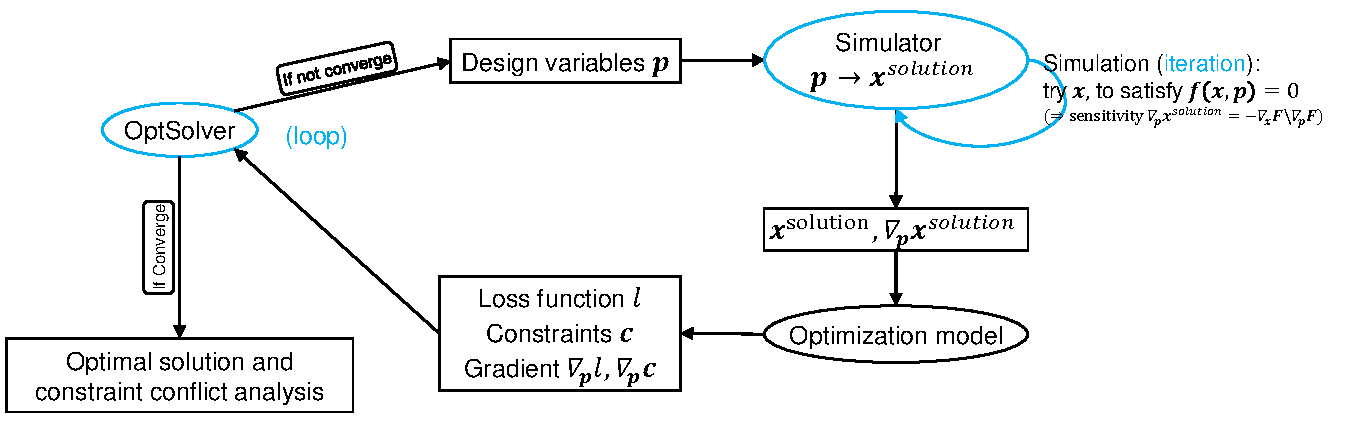
\includegraphics[width = 0.7\textwidth]{fig/solve-then-optimize.pdf}
  \caption{Automatic device sizing}
  \label{fig:solve-then-optimize}
\end{figure}

\begin{figure}[htbp]
  \centering
  \begin{subfigure}{0.3\textwidth}
    \includegraphics[width=\textwidth]{fig/amplifier-diagram.png}
    \caption{OpAmp schematic diagram \cite{OpAmpPNG}}
    \label{subfig:amplifier-diagram}
  \end{subfigure}
  \begin{subfigure}{0.65\textwidth}
    \includegraphics[width=\textwidth]{fig/amplifier-transfer-function.png}
    \caption{Input and output frequency response curves of the OpAmp after sizing}
    \label{subfig:amplifier-transfer-function}
  \end{subfigure}
  \caption{\textbf{(a)}: OpAmp schematic diagram, including the bias circuit and the main circuit, and a total of 17 n-MOSFET and 17 p-MOSFET devices. At the DC operating point, when small-signal disturbance with a given frequency is applied at $V_+,V_-$, an output signal is detected at $V_{out}$. \textbf{(b)}: Frequency response curves of OpAmp after sizing under $Corner=tt,Temperature=27$ conditions, where, va4 and va5 are the two internal nodes in the circuit.}
\end{figure}
Taking an OpAmp (Figure \ref{subfig:amplifier-diagram}) as an example, consider the design variables of the circuit (i.e., the channel length and width of each MOSFET) as the variables to be optimized.
Given the external current and voltage sources Ibias0, Ibias1, and $V_{dd},V_+,V_-$ and the load resistance and capacitance $R_L=200\Omega,C_L=10^{-10}\text{F}$, set the optimization goals as follows:
\begin{enumerate}[partopsep=0pt,topsep=0pt,itemsep=0pt,parsep=0pt]
  \item The DC operating points of all MOSFETs must be saturated under nine PVT conditions defined by $Corner\in[tt,ff,ss],Temperature\in[27,-40,125]$. For example, for an NMOS, its DC bias voltage must satisfy
    \vspace{-1em}
    \[
      \min(V_{gs},V_{ds},V_{sb},V_{gs}-V_{th})\geq0,
      \vspace{-1em}
    \]
    where, $V_{th}$ is subject to MosL,$V_{gs},V_{ds}$. For different PVT conditions, the SubModel needs to load different databases, and therefore the final simulation solutions obtained are also different.
  \item Under the typical condition of $Corner=tt,Temperature=27$, slight fluctuation is allowed for voltage sources $V_+,V_-$ as long as $V_++V_-=5v$ is satisfied. For the DC bias of $V_{out}$, the maximum must be greater than 4.35 V, and the minimum must be less than 0.3 V.
    Because our model (Section \ref{subsec:cmos-model}) is not used in the TRAN analysis, this requirement plays a similar role as the output swing indicator of circuits.
  \item AC analysis is performed on the circuit under the typical condition $Corner=tt$, $Temperature=27$ and a $v_{in+},v_{in-}=\pm0.5$ signal is applied at $V_+,V_-$. The DC gain $gain=20\cdot\log_{10}(|v_{out}|)$ of $V_{out}$ must reach 100.
  \item The design variables of each device meet given symmetry constraints. For example, the input MOSFET pair $M_{n0\_in},M_{n0\_ip}$ have the same size (MosL,MosW), and the current mirrors $M_{p30\_mirr},M_{p20\_mirr},M_{p10\_mirr},M_{p50\_mirr},M_{p60\_mirr}$ have the same channel length (MosL).
\end{enumerate}
\begin{equation}\label{eq:optimization}
  \begin{split}
    \min_{\bm{p}} l &= \max(5-\log_{10}(|\bm{v}[out]|),0)^2 \\
    \st \ \ \ \ \ \ 
    & \forall c\in[tt,ff,ss],t\in[27,-40,125], \\
    & \ \ \ \ \bm{x}_L\preceq\bm{x}^{c,t}\preceq\bm{x}_U;
    Saturation(\bm{x}^{c,t},\bm{p})\succeq\bm{0}; \\
    & \bm{x}^{down}[out]\leq0.3;\bm{x}^{up}[out]\geq4.35; \\
    & \bm{v}=\bm{A}^{tt,27}\backslash\bm{b}^{tt,27}; \ C\cdot\bm{p}=\bm{0}.
  \end{split}
\end{equation}
This design task can be expressed as a constrained optimization problem Prob.\eqref{eq:optimization}. $\bm{p}\to\{\bm{x}^{c,t}\},\bm{x}^{down},\bm{x}^{up}$ is obtained by solving the system of DC equations under corresponding PVT conditions with input bias $V_+,V_-$. And $\bm{v}=\bm{A}^{tt,27}\backslash\bm{b}^{tt,27}\triangleq\bm{A}\ \backslash\bm{b}$ solves the system of AC linear equations under the $Corner=tt$,$temperature=27$ condition, where the matrix elements of $\bm{A}$ are GM, GDS, etc. of each device subject to $\bm{x}^{tt,27},\bm{p}$. We can use a computational graph of mixed DCAC analysis to calculate $\bm{A},\bm{b},\nabla_{\bm{x}}\bm{A},\nabla_{\bm{x}}\bm{b}$ \footnote{$A=i\omega\cdot\nabla_{\bm{x}}\bm{Q}+\nabla_{\bm{x}}\bm{F}$. For a simpler graph implementation, use the DCAC computational graph (instead of $\nabla\bm{Q},\nabla\bm{F}$) to calculate $\nabla A$. This avoids calculating and propagating backward the second derivative of $\bm{Q},\bm{F}$ with regard to $\bm{x}$.}, which can further enable the calculation of $\nabla_{\bm{x}}l,\nabla_{\bm{p}}l$ (Appendix \hyperref[appendix:inv-linear-equation-grad]{C}). $C\cdot\bm{p}=\bm{0}$ represents the direct constraints on design variables, such as a symmetry constraint.

The optimization algorithm is implemented by using the open-source software Ipopt \cite{wachter2006implementation} and includes 72 variables, 27 equality constraints, and 308 inequality constraints to be solved. It took 356 seconds to run the whole process (including compiling Julia code and parsing netlist, etc.) on six threads on Intel(R) Core(TM) i7-8700 CPU at 3.20 GHz. Figure \ref{subfig:amplifier-transfer-function} shows the frequency response curve of the optimized circuit. The experimental results show that:
\begin{enumerate}[partopsep=0pt,topsep=0pt,itemsep=0pt,parsep=0pt]
  \item In hierarchical circuit simulation or sizing based on the computational graph, the device model and solution algorithm are decoupled from each other, allowing for high flexibility and efficiency.
  \item The parameters in the computational graph are processed to function as variables, making gradient optimization of many indicators simpler and easier.
\end{enumerate}
Note that the preceding experiments only consider the operation points of devices and circuit DC gains under typical conditions. To complete the design, more indicators (even discrete value indicators) need to be introduced into the optimization problem. There is no shortcut to properly integrating all indicators into the optimization framework, which however will not be addressed here.




